% !TEX root = ../gnss_interference_resistant_thesis.tex
\documentclass[main.tex]{subfiles}

\begin{document}

\subsection{GPS sistema}

GPS (angl. Global Positioning system), yra palydovais paremta navigacinė
sistema, priklausanti Jungtinėms Amerikos Valstijoms. Ši sistema yra viena
iš kelių globalių navigacinių (GNSS) sistemų. Naudojantis GPS sistema,
galima nustatyti vartotojo buvimo vietą (ilgumą, platumą, aukštį), bei
galima tiksliai susinchronizuoti laiką. Šiuo metu yra teikiamos dvi pasalugos:

\begin{itemize}
    \item Tikslaus pozicianavimo pasalauga (PPS)\cite{pps_standard}, skirta kariniam naudojimui
    \item Standartinė pozicianavimo pasalauga (SPS)\cite{sps_standard},
    atvira civiliniam naudojimui.
\end{itemize}

Šiame darbe bus nagrinėjami tik SPS signalai.

\subsubsection{Pozicijos ir laiko nustatymas}

Kad imtuvas galėtų nusistatyti savo poziciją, jam reikia priimti signalą bent
iš 4 palydovų. GPS signalas sudarytas taip, būtų galima išmatuoti atsumą iki
kiekvieno palydovo, signale yra užkoduodas iššiuntimo laikas, todėl priėmus
signalą iš paldydovo, žinant tikslų imtuvo laiką ($t_{imtuvo}$), sklidimo greitį ($c$),
iššsiuntimo laiką ($t_{siustuvo}$), galima išmatuoti signalo keliavimo trukmę ir suskaičiuoti
atsumą ($s$) iki palydovo:

\begin{equation}
    s = c * (t_{imtuvo} - t_{siustuvo})
\end{equation}

\subsubsection{GPS signalas}

Visi GPS palydovai siunčia apskiritimiškai polirizuotą signalą, trijose skkirtingose
dažnių juostose: L1 - $1575,42\ \mathrm{MHz}$, L2 - $1227,60\ \mathrm{MHz}$ ir
L5 - $1176,45\ \mathrm{MHz}$\cite{sps_standard}. Šiame darbe naudojimui pasirinktas
L1 signalas, kadangi jis yra palaikomas visų GPS palydovų, bei supaprastina imtuvų
konstrukciją, kadangi nereikia priimti signalų skirtingose dažnių juostose, todėl toliau
bus nagrinėjamas tik L1 signalas.

L1 signalo nešlys susideda iš dviejų komponentų kurių fazė skiriasi $90\degree$.
Kiekvienas nešlio komponentas yra faziškai moduliuojamas atskirų skaitmeninių signalų.
Primasis nešlio komonentas yra koduojamas P(Y) kodo ir LNAV duomenų (50 bitų/s) suma.
P(Y) kodas yra skirtas tikslios pozicijos nustatymui, ir šiuo metu jis yra užkuoduotas.
LNAV duomenys yra skirti, perduoti imtuvui tam tikrus GPS sistemos parameturus, tokius
kaip orbitos duomenis, laikrodžio korekcijos ir kita.
Antoji nešlio dalis yra moduliuojama C/A (netikslaus sekimo) kodu ir tais pačiai LNAV
duomenimis. C/A kodas yra 1023 "čirpų" ilgio ir jo dažnis yra $1.023\ \mathrm{MHz}$.
C/A kodas yra naudojamas signalo sklidimo trukmei matuoti.

\begin{figure}[h]
    \begin{centering}
    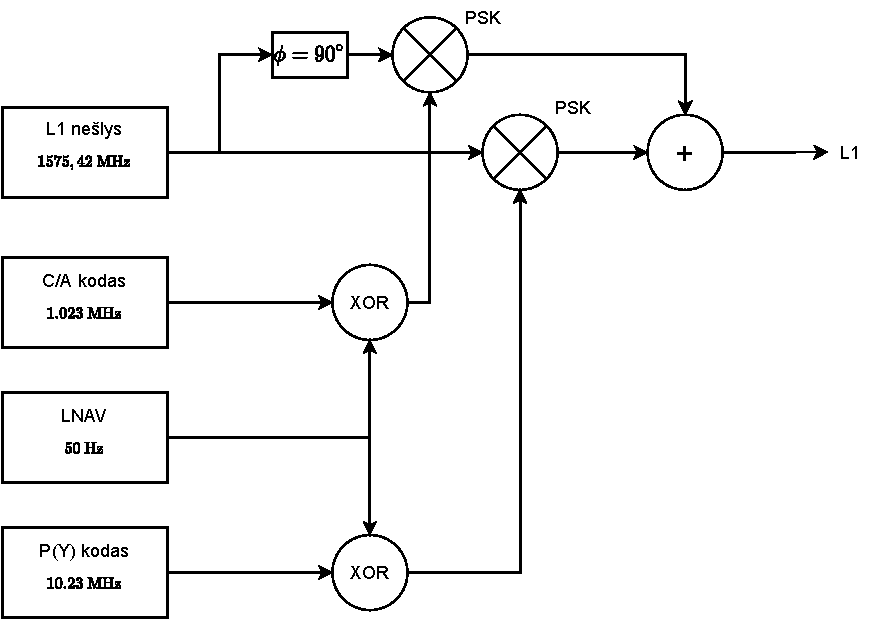
\includegraphics[scale=0.85]{drawings/l1_signal}
    \par\end{centering}
    \protect\caption{\label{fig:l1_signal}L1 signalo moduliatoriaus schema. Adaptuota iš \cite{Sadeghi2008TimeSS}.}
\end{figure}

Kadangi visi palydovai transliuoja tuo pačiu dažniu, C/A kodas pasirenkamas toks,
kad jis būtų pseudo-atsitiktinis kodas (PRN), kiekvienam palydovui yra suteiktia unikali seka.
Svarbiausia PRN savybė, ir ta, kad autokoreliacijos rezultato maksimumas yra tik
ties 0 tašku \cite{OCHIN202121_chapter2}.

Imtuvai ieškodami paldyvo signalo, susigeneruoja ieškomo paldyovo unikalią C/A signalo
kopiją ir atlieka koreliaciją tarp lokaliai sugeneruoto signalo ir priimto.
Iš gauto koreliaicjos rezultato galima nustatyti gauto C/A signalo užlaikymą.

\subsubsection {GPS paklaidos}

Atliekami GPS signalo matavimai yra veikiami skirtingų tipų atstiktinių ir sistematinių
paklaidų. Paklaidas galima suskirstyti į kelias pagrindines katergorijas\cite{KUMAR20213_chapter1}:

\begin{itemize}
    \item Pladyovo ir imtuvo laikrdožio paklaidos
    \item Atspindžių paklaidos
    \item Atmosferinės paklaidos
    \item Orbitos paklaidos
\end{itemize}

Paldyduovuose naudojami atominiai laikrodžiai yra labai tikslūs, tačiau visi vien atsiranda paklaidos.
Tipinė palydovo laikrodžio paklaida yra $8-17\ \mathrm{ns}$ per dieną. Tokios paklaidos
gali būti elimituotos priimtant signalą iš kelių paldyvoų. Dėl laikrodžio netikslumų atsiranda
pozicijos paklaidos iki kelių metrų \cite{KUMAR20213_chapter1}.

GPS signalų saveika su aplinka, pastatais, reliefu, sukelia atspindžių paklaidas. Kadangi
atsipindėjęs signalas nukeliauja didesnį atstumą, naudojantis tokiu signalu nebeįmanoma
tiksliai nustatyti atsumo iki palydovo, ko pasekoje mažėja galutinės pozicijos tikslumas.

Atmosferinės paklaidos atsiranda dėl radijo bangų sklidimo parametrų kitimo atmosferoja ir
jonosferoje. Kadangi parametrai pastoviai kinta laike, dėl besikeičiančių atmosfers/jonosferos
sąlygų. Dėl šių veiksnių atsiradusios paklaidos yra didžiausios lyginant su kitomis.
Šių trigžių šalinimas įmanomas pasinaudojant korekcijomis iš antžeminių stočių, taip
pat galima priiminėti L1 ir L5 signalus. Kadangi šie signalai veikia skirtinguose
dažnių ruožuose, atmosferos reiškiniai juos veikia skirtingai, todėl galima pašalinti
paklaidas.

Kadani orbitoje esantys paldyovai yra veikiami nenuspėjamų jėgų, bėgant laikui jų orbitos
po truputį keičiasi. Norint pašalinti šias paklaidas, visi palydovai transliuoja savo
orbitos duomenis, ir juos atnaujina kas 4 valandas \cite{sps_standard}. Paldyovų orbitas
matuoja antžeminės GPS sistemos valdymo stotys, kurios perduoda šiuos duomenis
į palydovus, kad šie galėtų juos išsųsti imtuvams per LNAV žinutes.

\end{document}
